\section{Outside parts}\label{sec:count}

Let $W$ be a subgraph of a graph $G$. Put $r=\beta(G)$, $t=\beta(W)$ and $m=|E(W)|$. The map
$\xi\mapsto\xi\sm E(W)$ is linear on $\Z(G)$, and its kernel is $\Z(W)$. So there are $2^{r-t}$
outside parts, and each of them is the outside part of exactly $2^{t}$ even subgraphs. If $\xi$ is
uniform on $\Z(G)$, then its outside part is uniform on the set of outside parts. Let
\[
  p(G,W)=\PP\bigl(\xi\sm E(W)\text{ is a forest}\bigr).
\]
This is the proportion of outside parts that are forests. It is also the proportion of even
subgraphs whose outside part is a forest:
\begin{equation}\label{eq:count}
  \bigl|\{\xi\in\Z(G):\ \xi\sm E(W)\text{ is a forest}\}\bigr|\;=\;p(G,W)\,2^{r}.
\end{equation}

\begin{lemma}[Counting lemma]\label{lem:count}
Let $p=p(G,W)$.
\begin{enumerate}
\item[\textup{(a)}] If a cycle $C$ of $G$ contains an edge of $W$, then $C\sm E(W)$ is a forest.
Hence at most $p\,2^{r}$ cycles of $G$ contain an edge of $W$.
\item[\textup{(b)}] The cycles of $G$ have at most $2^{r-t}\bigl(pm+1-p\bigr)$ different lengths.
\end{enumerate}
\end{lemma}

\begin{proof}
(a) A proper subset of the edge set of a cycle contains no cycle. The second statement follows
from~\eqref{eq:count}, because distinct cycles are distinct even subgraphs.

(b) Let $x$ be an outside part. Suppose first that $x$ is not a forest, and let $C$ be a cycle with
outside part $x$. Then $x$ contains a cycle and $x\subseteq C$, which forces $C=x$. So $x$ accounts
for at most one cycle, and hence for at most one length. Now suppose that $x$ is a forest, and let
$C$ be a cycle with outside part $x$. Then $C$ contains an edge of $W$, because $C$ is not a
forest. The length of $C$ is $|x|+|C\cap E(W)|$, and $1\le|C\cap E(W)|\le m$. So $x$ accounts for
at most $m$ lengths. There are $p\,2^{r-t}$ outside parts that are forests and $(1-p)\,2^{r-t}$
that are not.
\end{proof}

If $W$ has at least one edge, then part~(b) with $p\le1$ gives the bound~\eqref{eq:trivial} of the
introduction. The lemma improves on it when $p$ is less than one.

\begin{example}[Two points of attachment]\label{rem:twoports}
Suppose that $G=W\cup N$, where $W$ and $N$ are connected, have no common edge, and have exactly two
common vertices $u$ and $v$. A \emph{$\{u,v\}$-join} of $N$ is a set of edges of $N$ in which $u$
and $v$ have odd degree and all other vertices have even degree. The outside parts are the
$2^{\beta(N)}$ even subgraphs of $N$ and the $2^{\beta(N)}$ joins of $N$. A nonempty even subgraph
is not a forest. Hence
\[
  p(G,W)\;\le\;\frac{1+2^{\beta(N)}}{2^{\beta(N)+1}}\;=\;\frac12+2^{-\beta(N)-1},
\]
with equality if and only if every join of $N$ is a forest. So when $W$ is attached at two
vertices, the error term in~\eqref{eq:forest} can be replaced by $2^{-\beta(N)-1}$, which is
exponentially small.

For a concrete case, let $N$ be a chain of $k$ four-cycles, each joined to the next at opposite
vertices, and let $u$ and $v$ be the two ends of the chain. Every join of $N$ is a path from $u$ to
$v$, so equality holds. If $W$ is a triangle and $k$ is large, this graph satisfies the hypotheses
of Theorem~\ref{thm:forest}. So the constant $\half$ in~\eqref{eq:forest} cannot be lowered.

Figure~\ref{fig:twoports} shows the case $k=2$. There $\beta(G)=4$ and $\beta(N)=2$. The eight
outside parts are the four even subgraphs of $N$ and the four paths from $u$ to $v$ in $N$. Five of
them are forests, so $p(G,W)=5/8$. Lemma~\ref{lem:count}(a) allows $\frac58\cdot16=10$ cycles
through $W$, and there are nine.
\end{example}

\begin{figure}[ht]
\centering
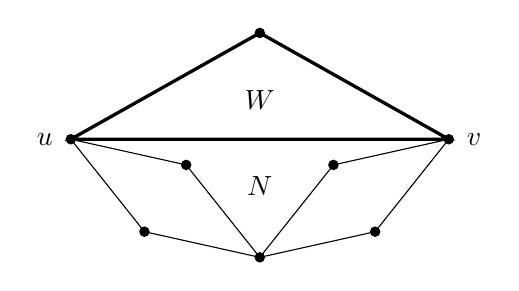
\begin{tikzpicture}
  \coordinate (s) at (0,0);
  \coordinate (t) at (4.8,0);
  \coordinate (m) at (2.4,-1.5);
  \coordinate (w) at (2.4,1.35);
  \coordinate (x1) at (1.465,-0.326);
  \coordinate (y1) at (0.935,-1.174);
  \coordinate (x2) at (3.335,-0.326);
  \coordinate (y2) at (3.865,-1.174);
  \draw (s)--(x1)--(m)--(y1)--cycle;
  \draw (m)--(x2)--(t)--(y2)--cycle;
  \draw[very thick] (s)--(w)--(t)--cycle;
  \foreach \p in {s,t,m,w,x1,y1,x2,y2} \fill (\p) circle (1.9pt);
  \node[left=3pt] at (s) {$u$};
  \node[right=3pt] at (t) {$v$};
  \node at (2.4,0.5) {$W$};
  \node at (2.4,-0.6) {$N$};
\end{tikzpicture}
\caption{The graph of Example~\ref{rem:twoports} for $k=2$: a triangle $W$ (thick) and a chain $N$
of two four-cycles.}
\label{fig:twoports}
\end{figure}

